\documentclass[serif,aspectratio=169]{beamer}
\usepackage{fontspec,xunicode,xltxtra}
\usepackage{hyperref}
\usepackage{amsmath,amssymb,amsfonts,amsthm}
\usepackage{graphicx}
\usepackage{wasysym}            % male and female symbols
\usepackage{listings}

\usefonttheme{professionalfonts}

\XeTeXlinebreaklocale zh
\XeTeXlinebreakskip = 0pt plus 1pt minus 0.1pt

\setmainfont{FangSong}
\renewcommand{\baselinestretch}{1.25}

\AtBeginSection[]
{
  \begin{frame}
    \frametitle{目录}  %\insertsection to display section title                                                                             
    \tableofcontents[currentsection]
  \end{frame}
}

\AtBeginSubsection[]
{
  \begin{frame}
    \frametitle{目录}  %\insertsection to display section title                                                                             
    \tableofcontents[currentsubsection]
  \end{frame}
}

\addtobeamertemplate{navigation symbols}{}{%
  \usebeamerfont{footline}%
  \usebeamercolor[fg]{footline}%
  \hspace{1em}%
  \insertframenumber/\inserttotalframenumber
}
%\setbeamercovered{invisible}

\begin{document}

\title{\fontspec{LiSu}第一天:育种值估计概览}
\author{于希江}
\date{\tiny{~{二〇一八·十一月} \\青岛}}
\institute{挪威生命科学大学畜牧与水产系}
\titlegraphic{
\includegraphics[height=.1\textwidth]{img/nmbu.png}}

\frame{
  \titlepage
}


\section{育种和育种值}
\begin{frame}
  \frametitle{动物生产}
  \begin{columns}
    \begin{column}{.5\textwidth}
      \begin{description}
      \item [种] 育种和遗传。
      \item [料] 饲料配方和工艺。
      \item [病] 卫生防疫,疫病控制。
      \item [管] 动物生产系统管理。
      \end{description}
    \end{column}

    \pause
    \begin{column}{.5\textwidth}
      \begin{itemize}
      \item 肉鸡 1957,2001 品系交叉饲喂同期饲料胴体重对比\tiny{(公鸡,克;43, 57, 71, 和 85 天结果。Havenstein et al, 2003.)}:
%        \begin{center}
%          \begin{tabular}{cc|rrrr}
%            品系 & 饲料 & 43d & 57d & 71d & 85d\\\hline
%            2001 & 2001 & 2,078 & 3,145 & 3,938 & 4,591\\
%            2001 & 1957 & 1,536 & 2,207 & 2,874 & 3,494\\
%            1957 & 2001 &   391 &   632 &   882 & 1,216\\
%            1957 & 1957 &   340 &   535 &   790 & 1,101
%          \end{tabular}
        %        \end{center}
      \end{itemize}
      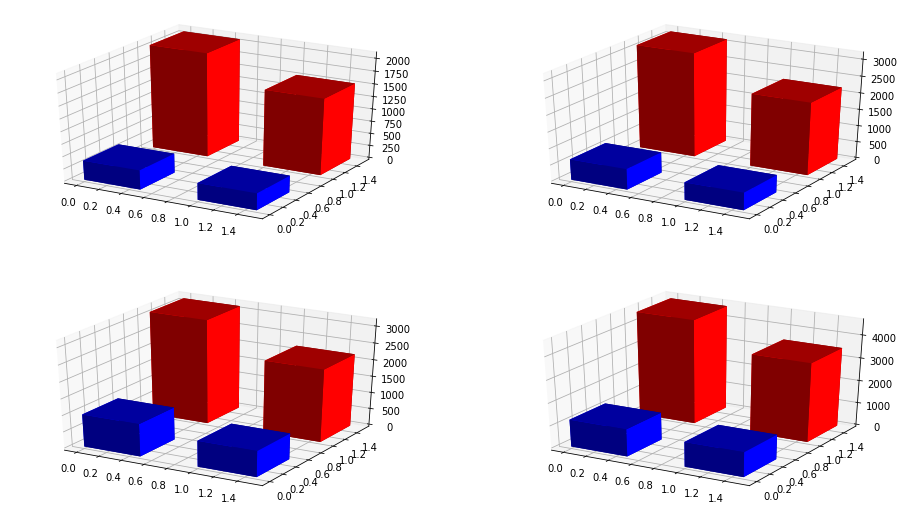
\includegraphics[width=\textwidth]{img/chicken.png}
    \end{column}
  \end{columns}
\end{frame}


\begin{frame}
  \frametitle{育种的流程}
  \centering
  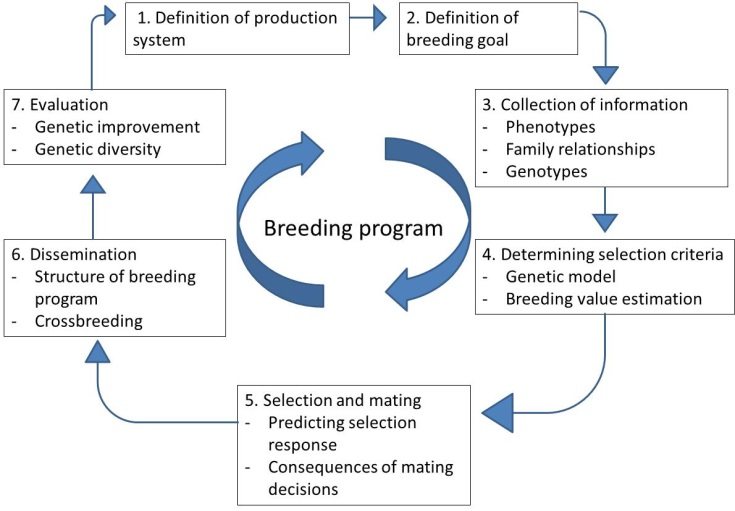
\includegraphics[width=.8\textwidth]{img/Breeding-program.jpg}
\end{frame}


\begin{frame}
  \frametitle{育种的流程}
  \begin{columns}
    \begin{column}{.36\textwidth}
      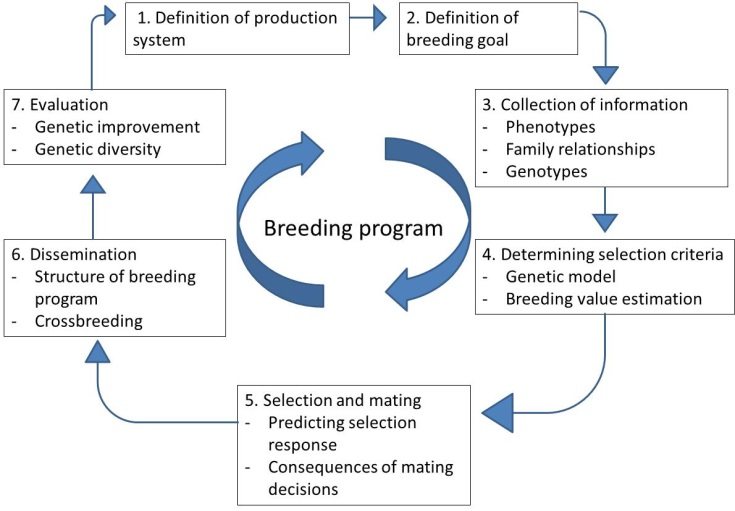
\includegraphics[width=\textwidth]{img/Breeding-program.jpg}
      \begin{itemize}
      \item 摘自 \tiny{\url{https://wiki.groenkennisnet.nl/display/TAB}}
      \end{itemize}
    \end{column}
    \begin{column}{.32\textwidth}
      \begin{itemize}
      \item 确定生产系统
      \item 确定育种目标
      \item 收集信息
        \begin{itemize}
        \item 表型
        \item 系谱资料
        \item {\color{cyan}基因型}
        \end{itemize}
      \item 确定选择标准
        \begin{itemize}
        \item 遗传模型
        \item 育种值估计
        \end{itemize}
      \end{itemize}
    \end{column}
    \begin{column}{.32\textwidth}
      \begin{itemize}
      \item 选择和交配
        \begin{itemize}
        \item 预测选择反应
        \item 交配结果的预后
        \end{itemize}
      \item 传播
        \begin{itemize}
        \item 育种项目的结构
        \item 杂交
        \end{itemize}
      \item 评估
        \begin{itemize}
        \item 遗传改良
        \item 遗传多样性
        \end{itemize}
      \end{itemize}
    \end{column}
  \end{columns}
\end{frame}


%注意:这一天的内容就是要理解育种值,
%      了解为什么要通过模型来理解育种值
\begin{frame}
  \frametitle{育种和育种值}
  \begin{columns}
    \begin{column}{.5\textwidth}
      \begin{block}{育种的定义}
        \hspace{2em}指在一个群体中,在控制{\color{cyan}近交}的情况下获得{\color{cyan}遗传进展}。
      \end{block}
      \begin{block}{有关遗传进展}
        $$\Delta G = \frac{ir\sigma_a}{L}$$
      \end{block}
    \end{column}
    \pause
    \begin{column}{.5\textwidth}
      \begin{block}{育种值定义(之一)}
        \hspace{2em}一个特定群体中,如果一个个体可以与该群体中的个体随机交配产生后代,那么这些{\color{cyan}后代}在某个性状上的表型的{\color{cyan}平均值}与群体平均数{\color{cyan}差异的二倍},就是{\color{cyan}该个体}在{\color{cyan}该群体}中关于{\color{cyan}该性状}的育种值。
      \end{block}
      \pause
      
      \begin{block}{育种值的估计}

        \vspace{-6ex}
        
        \begin{align*}
          P&=G+E\\
          &=\overbrace{A+D+I}^G+\overbrace{E_C+E_S}^E\\
          \overline{P}&=\overline{G}\quad\Leftarrow\overline{E}=0
        \end{align*}
        % 注意:育种值的估计并非不可以从后代测量,实际上传统上奶牛选择的是公牛
        % 只有女儿才有产奶记录,这样对公牛的选择要等到女儿有成绩后才能进行
        % 育种值估计。使得世代间隔长达近 7 年。
      \end{block}
    \end{column}
  \end{columns}
\end{frame}


\section{从加性遗传模型理解育种值}
\begin{frame}
  \frametitle{加性遗传模型}
  \begin{columns}
    \begin{column}{.5\textwidth}
      \begin{align*}
        P&=G+E\\
        &=\overbrace{A+D+I}^G+\overbrace{E_C+E_S}^E\\
        e_i&\stackrel{\mathrm{iid}}{\sim}N(0,\,\sigma^2)
      \end{align*}
      
%       \pause
%       \begin{itemize}
%       \item 它是错的
%         \begin{itemize}
%         \item Essentially, all models are wrong,
%         \end{itemize}
%         \pause
%       \item 但,它是非常有用的
%         \begin{itemize}
%         \item but some are useful.\\
%           \flushright{-- George Box}
%         \end{itemize}
%       \end{itemize}
    \end{column}

    \pause
    \begin{column}{.5\textwidth}
      \begin{itemize}
      \item 有了该模型,我们可以:利用系谱或者基因组数据估计育种值
        \begin{itemize}
        \item 模拟产生数据集 $D$
          \begin{itemize}
          \item 包括系谱、基因型和表现型
          \end{itemize}
        \item 尝试用若干种统计方法分析 $D$
          \begin{itemize}
          \item 估计育种值
          \item 利用常用的统计软件如 (Jupyter + Python)
          \item 多次模拟,评估估计效果
          \item 选项:估计遗传力
          \end{itemize}
        \end{itemize}
      \end{itemize}
    \end{column}
  \end{columns}
\end{frame}


\begin{frame}
  \frametitle{理解统计模型和一般估计方法}
  \begin{itemize}
  \item 要了解的概念
    \begin{itemize}
    \item 随机数
    \item 模型/建模
    \item 方程组
    \item 普通最小二乘
    \end{itemize}
  \end{itemize}
\end{frame}


\subsection{随机数}
\begin{frame}
  \frametitle{随机数}
  \begin{itemize}
  \item 真随机数,如:
    \begin{itemize}
    \item 一些物理现象
      \begin{itemize}
      \item 盖革计数器相邻两个声音的间隔时间
      \item 大气噪声(例如:\url{https://random.org})
      \end{itemize}
    \item 现在大部分 Linux/Unix 机器:/dev/urandom
    \end{itemize}
  \item 伪随机数,如:
    \begin{itemize}
    \item 线性同余发生器
      \begin{itemize}
      \item $N_{i+1} = (A\cdot N_i+B) \mod M$
      \item 如 glibc: $N_{i+1} = (1103515245\times N_i+12345)\mod 2^{32}$
      \end{itemize}
    \item mt19937
    \end{itemize}
  \end{itemize}
\end{frame}


\begin{frame}
  \frametitle{均匀分布}
  \begin{columns}
    \begin{column}{.5\textwidth}
      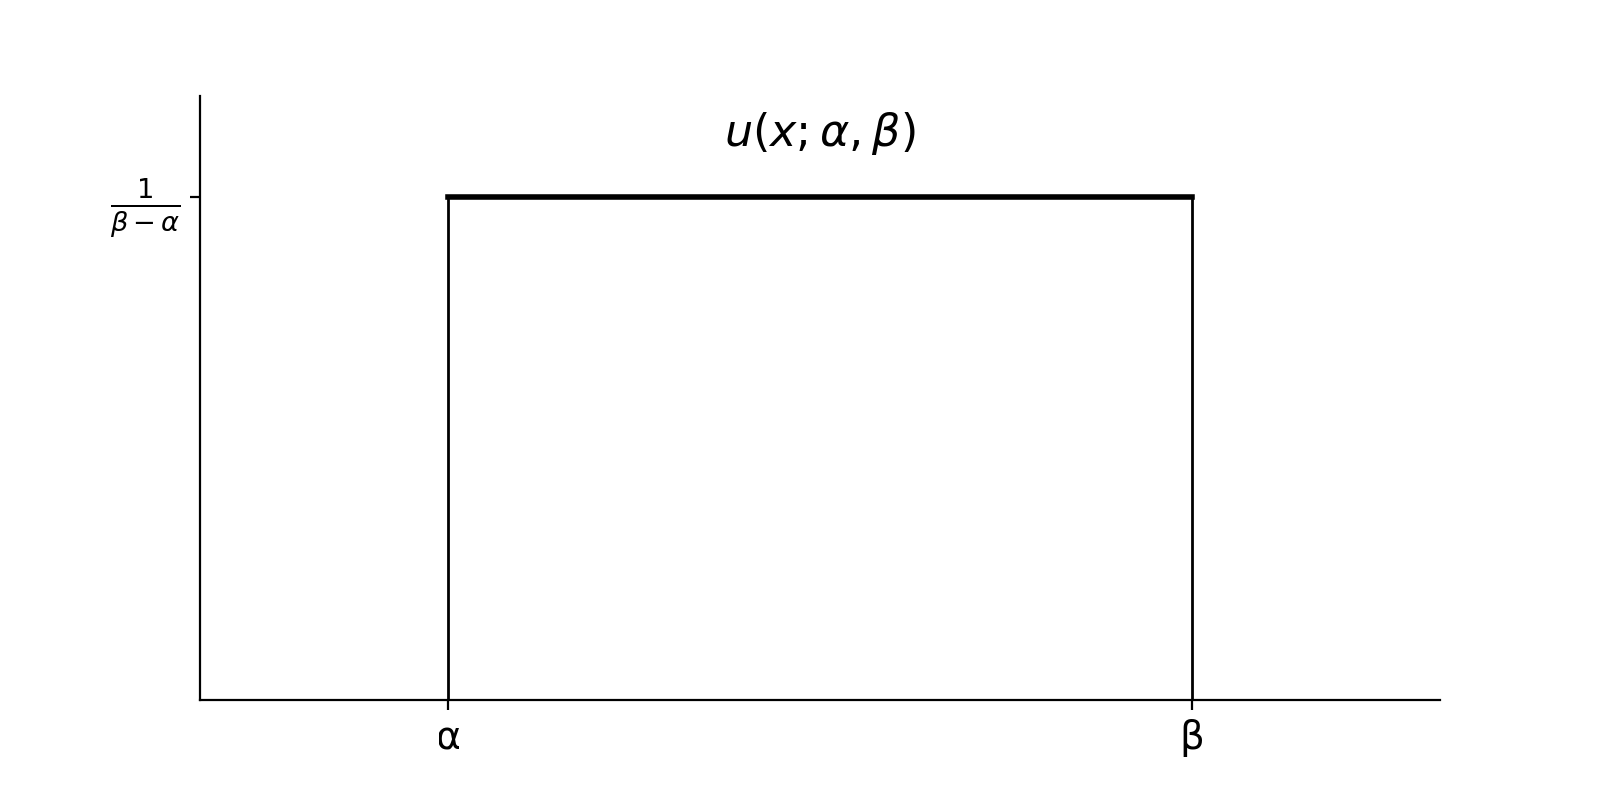
\includegraphics[width=\textwidth]{img/uniform.png}
    \end{column}
    \begin{column}{.5\textwidth}
      \begin{itemize}
      \item 均匀分布概率密度函数
      \end{itemize}
      
      $$u(x;\alpha,\beta) = \left\{\begin{array}{cl}\frac{1}{\beta-\alpha}&\textrm{for }\alpha<x<\beta\\0&\mathrm{elsewhere}\end{array}\right.$$
      
    \end{column}
  \end{columns}
 \end{frame}


\begin{frame}
  \frametitle{均匀分布随机数示例}
  \begin{columns}
    \begin{column}{.5\textwidth}
      \centering
      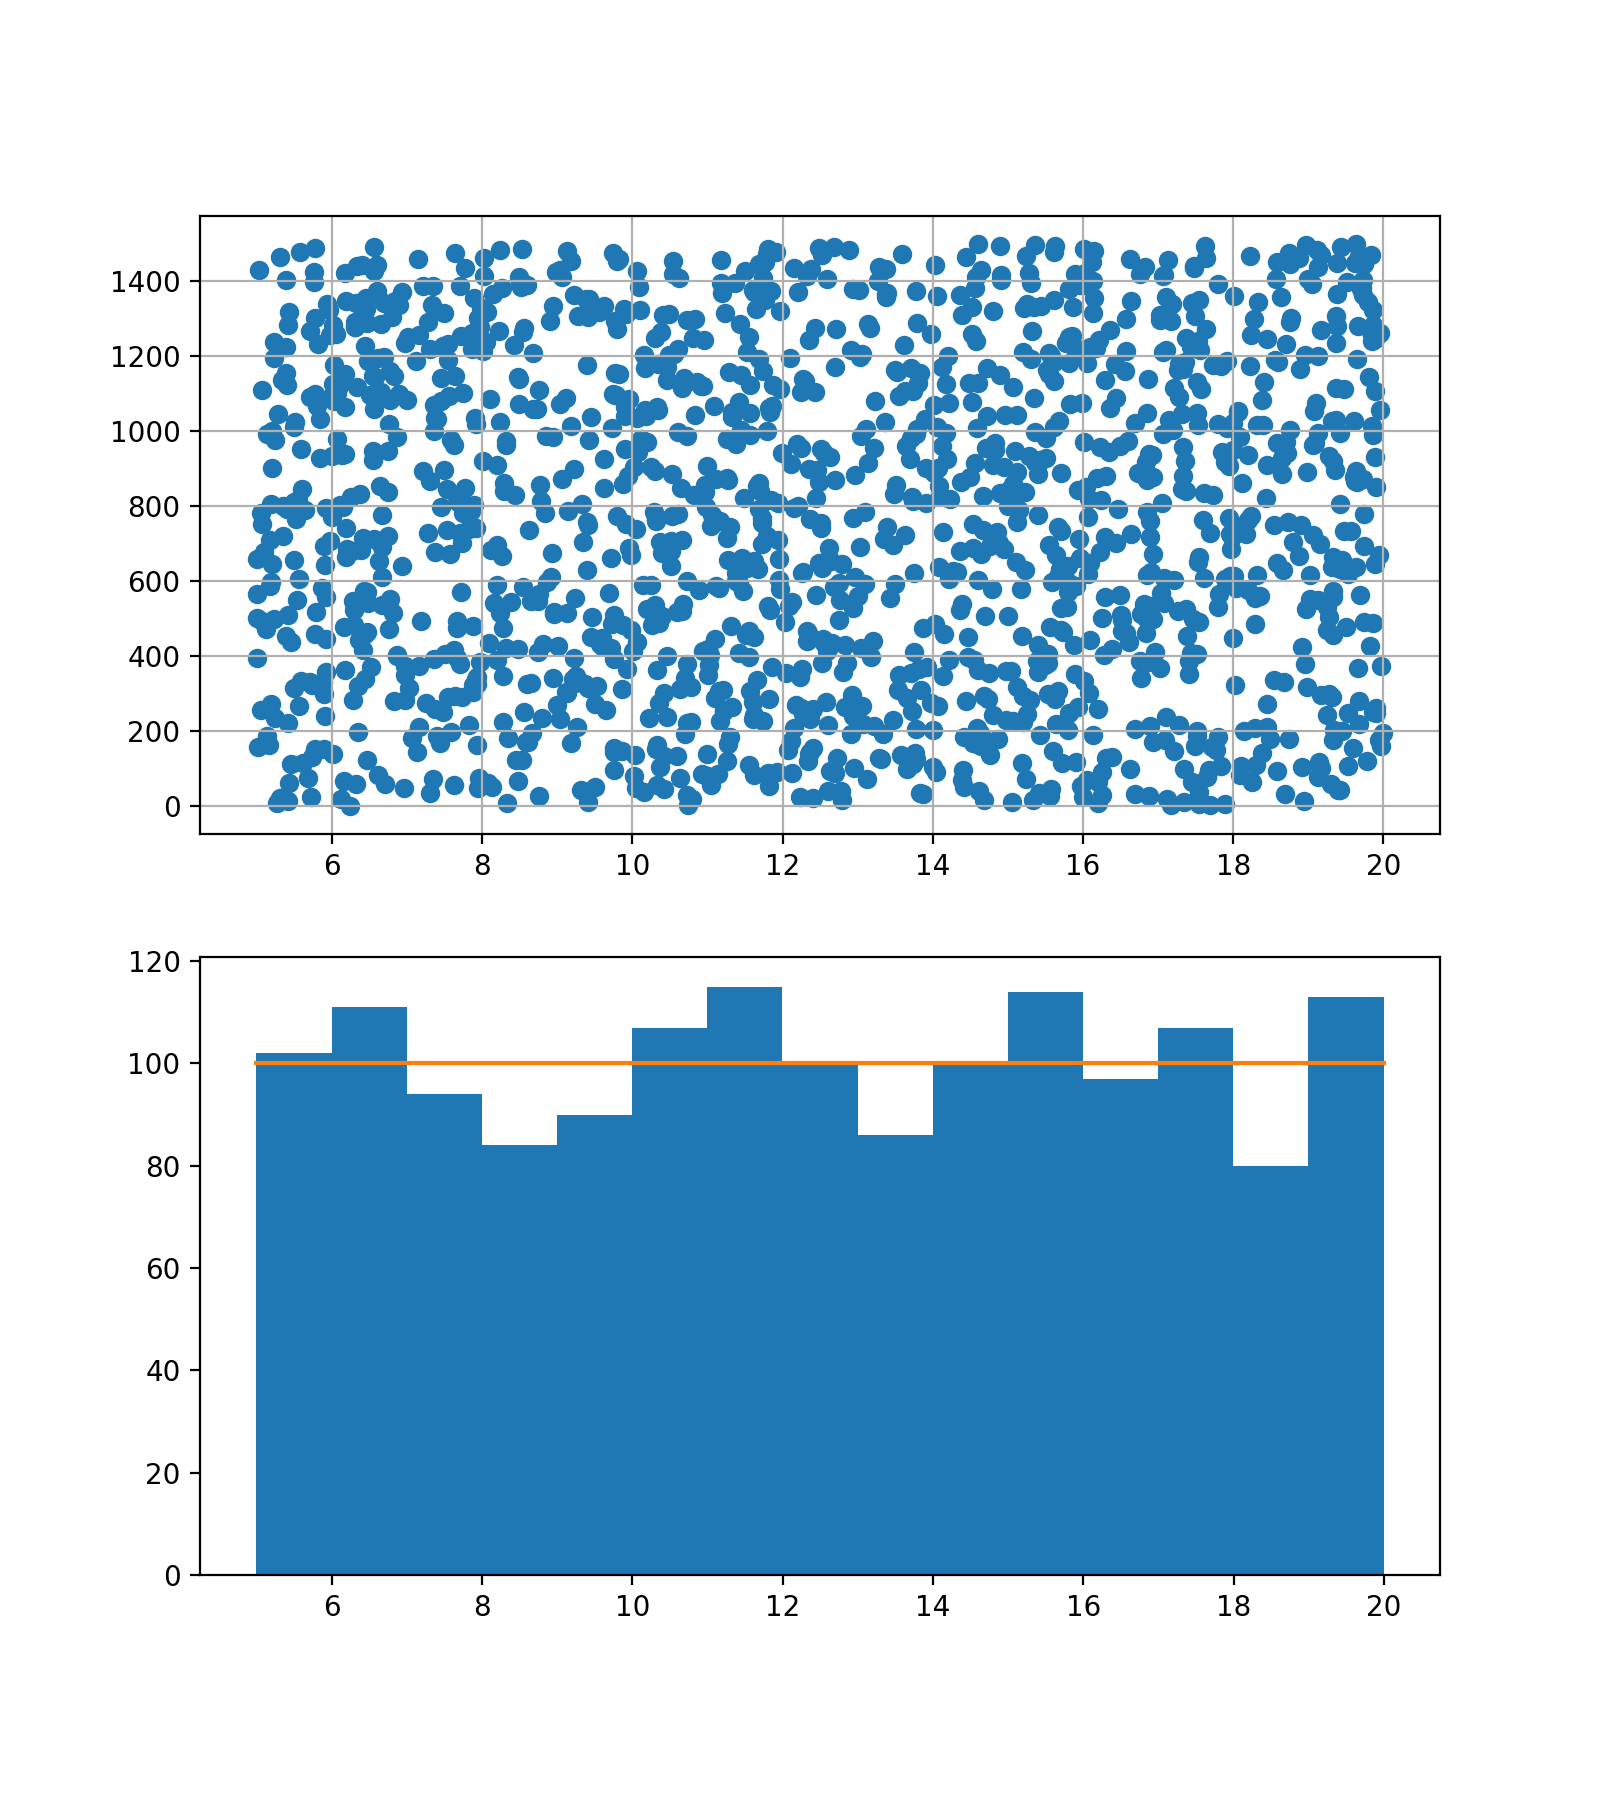
\includegraphics[width=.9\textwidth]{img/runif.png}
    \end{column}
    \begin{column}{.5\textwidth}
      \begin{itemize}
      \item 1,500 均匀分布随机数 $r\sim U(5,20)$
        \begin{itemize}
        \item 上图:1,500 点的散点图
        \item 下图:柱形图
        \end{itemize}
      \end{itemize}
    \end{column}
  \end{columns}
\end{frame}


\begin{frame}
  \frametitle{蒙特·卡罗模拟一例}
  \begin{columns}
    \begin{column}{.5\textwidth}
      \begin{itemize}
      \item 模拟用的均匀分布随机数需要
        \begin{itemize}
        \item 发生速度快
        \item 长周期(mt19937: $2^{19937}-1$)
        \item 相邻的 $n$ 个数字应尽可能均匀分布于每维 $\alpha$ 到 $\beta$ 的 $n$ 维空间。
        \item 其它
        \end{itemize}
      \item 如若 $x_i\sim U(0,1)$ 则点 $(x_{2i},\,x_{2i-1})$ 均匀分布在以 (0, 0) 到 (1, 1) 为对角线的正方形中。
      \item 于是,落入右图阴影部分的面积是 $\pi/4$。
      \item 见 {\small\color{cyan}day-1-some-random-numbers.ipynb}
      \end{itemize}
    \end{column}
    \begin{column}{.5\textwidth}
      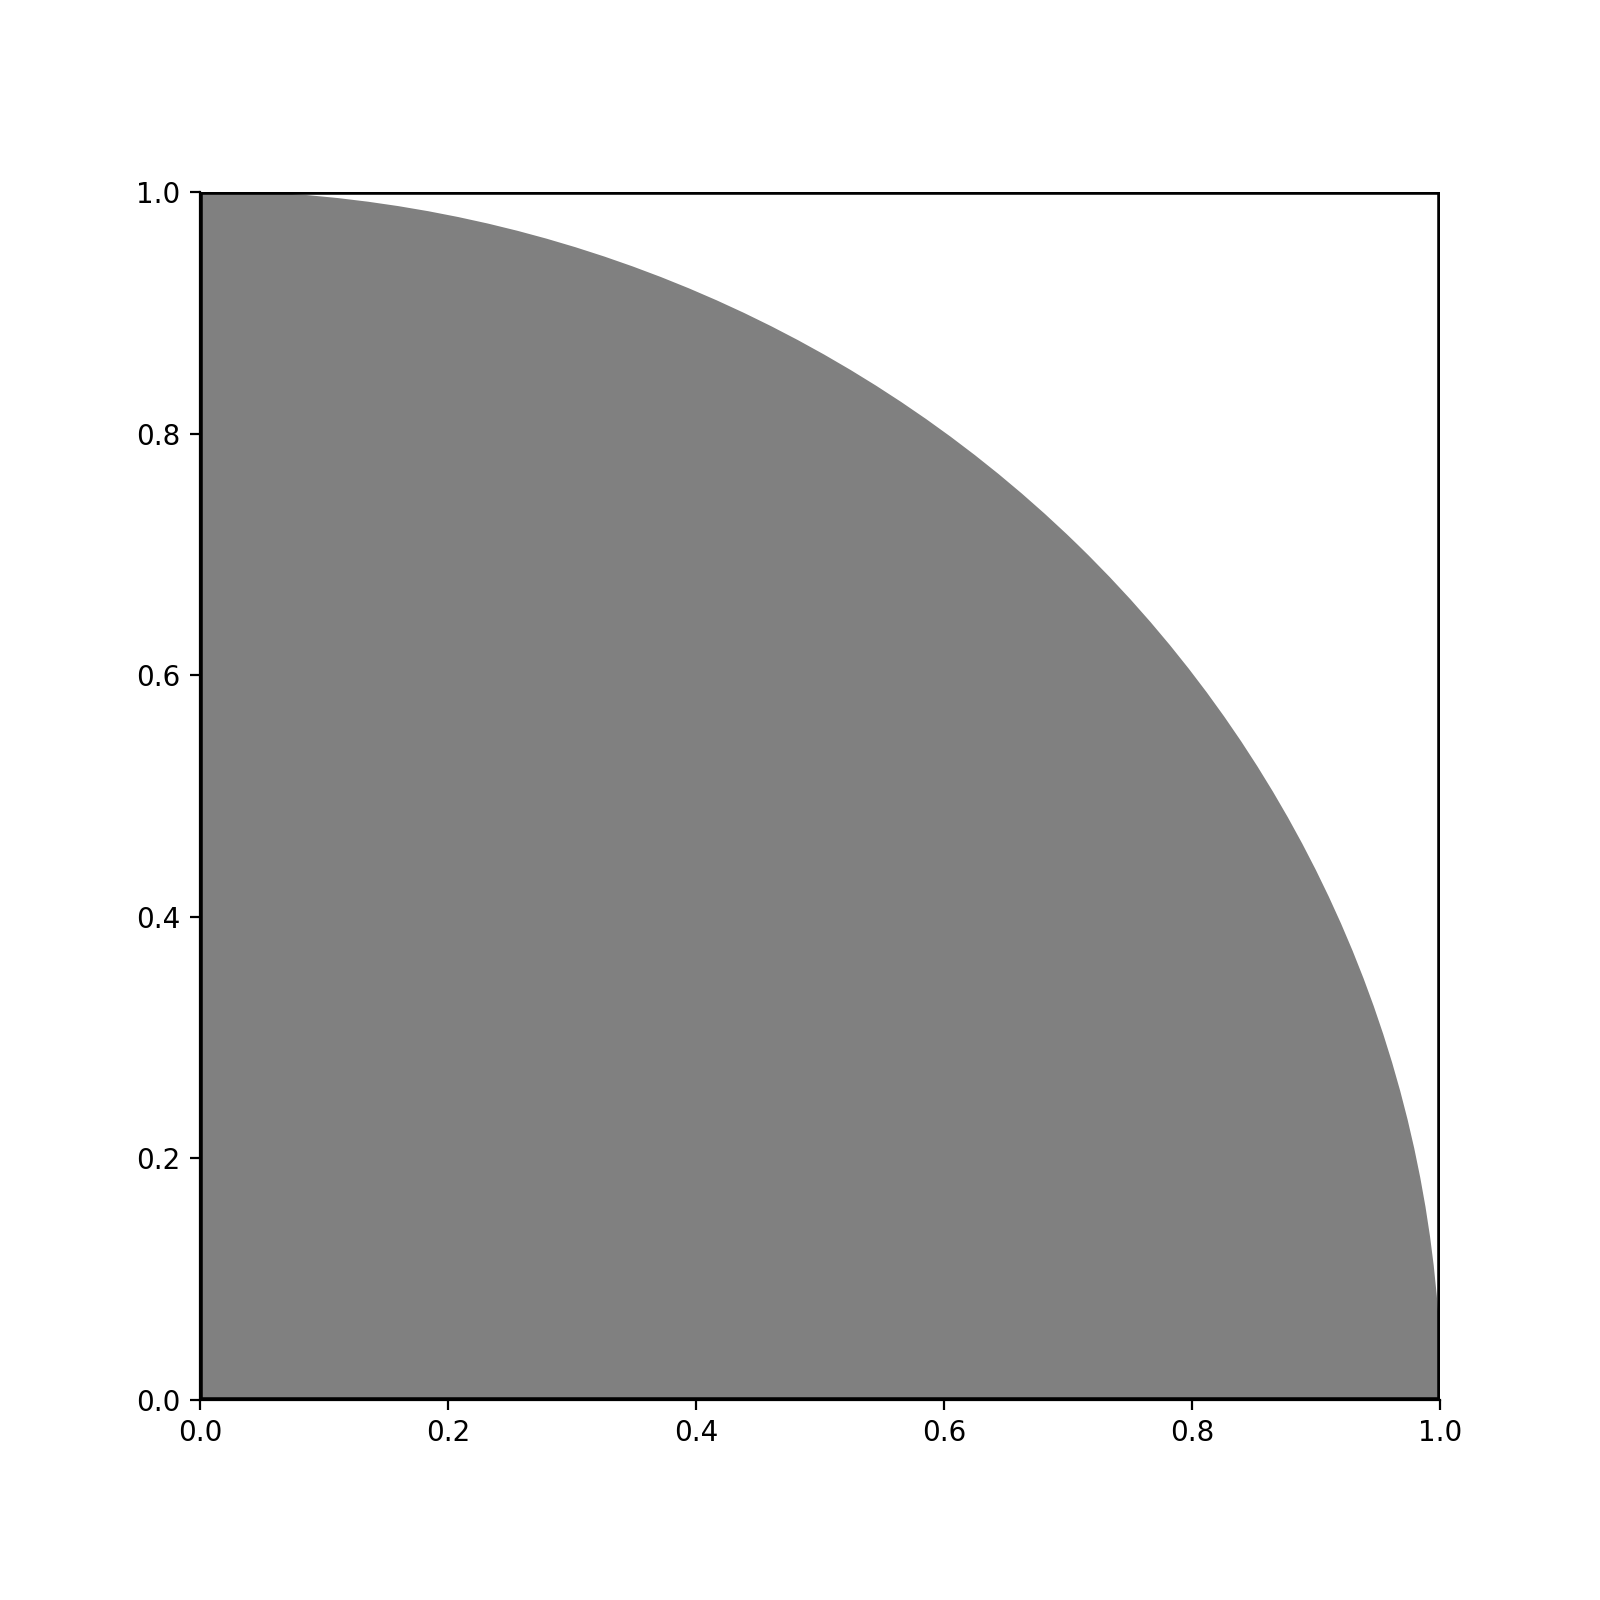
\includegraphics[width=\textwidth]{img/quarterCircle.png}
    \end{column}
  \end{columns}
\end{frame}


\begin{frame}
  \frametitle{正态分布}
  \begin{columns}
    \begin{column}{.5\textwidth}
      \centering
      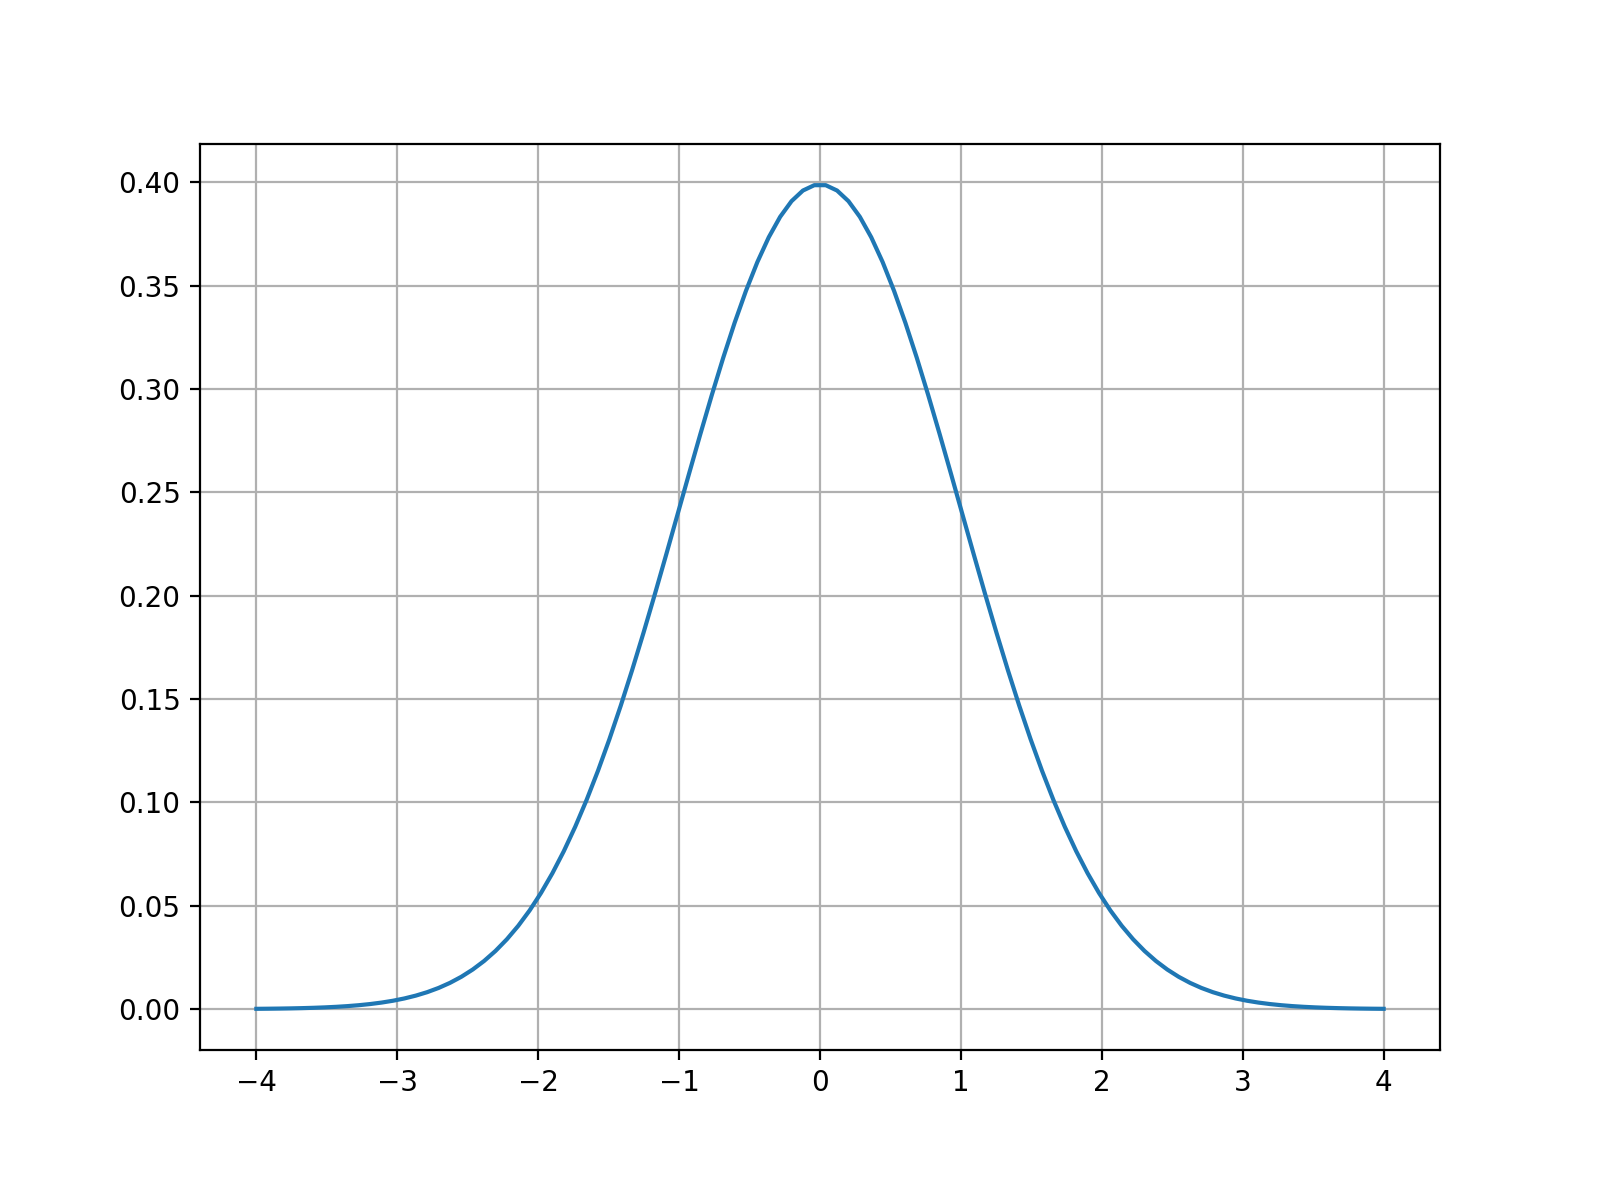
\includegraphics[width=.9\textwidth]{img/normal.png}
    \end{column}

    \begin{column}{.5\textwidth}
      \begin{itemize}
      \item 正态分布概率密度函数
      \end{itemize}
      $$n(x;\mu,\sigma)=\frac{1}{\sigma\sqrt{2\pi}}e^{-\frac{1}{2}\left(\frac{x-\mu}{\sigma}\right)^2}\quad x\in(-\infty,\,\infty)$$
    \end{column}
  \end{columns}
\end{frame}


\begin{frame}
  \frametitle{正态分布随机数示例}
  \begin{columns}
    \begin{column}{.5\textwidth}
      \begin{itemize}
      \item 1,000 个标准正态分布随机数 $r\sim U(5,20)$
        \begin{itemize}
        \item 上图:散点图
        \item 下图:柱形图
        \end{itemize}
      \end{itemize}
    \end{column}
    \begin{column}{.5\textwidth}
      \centering
      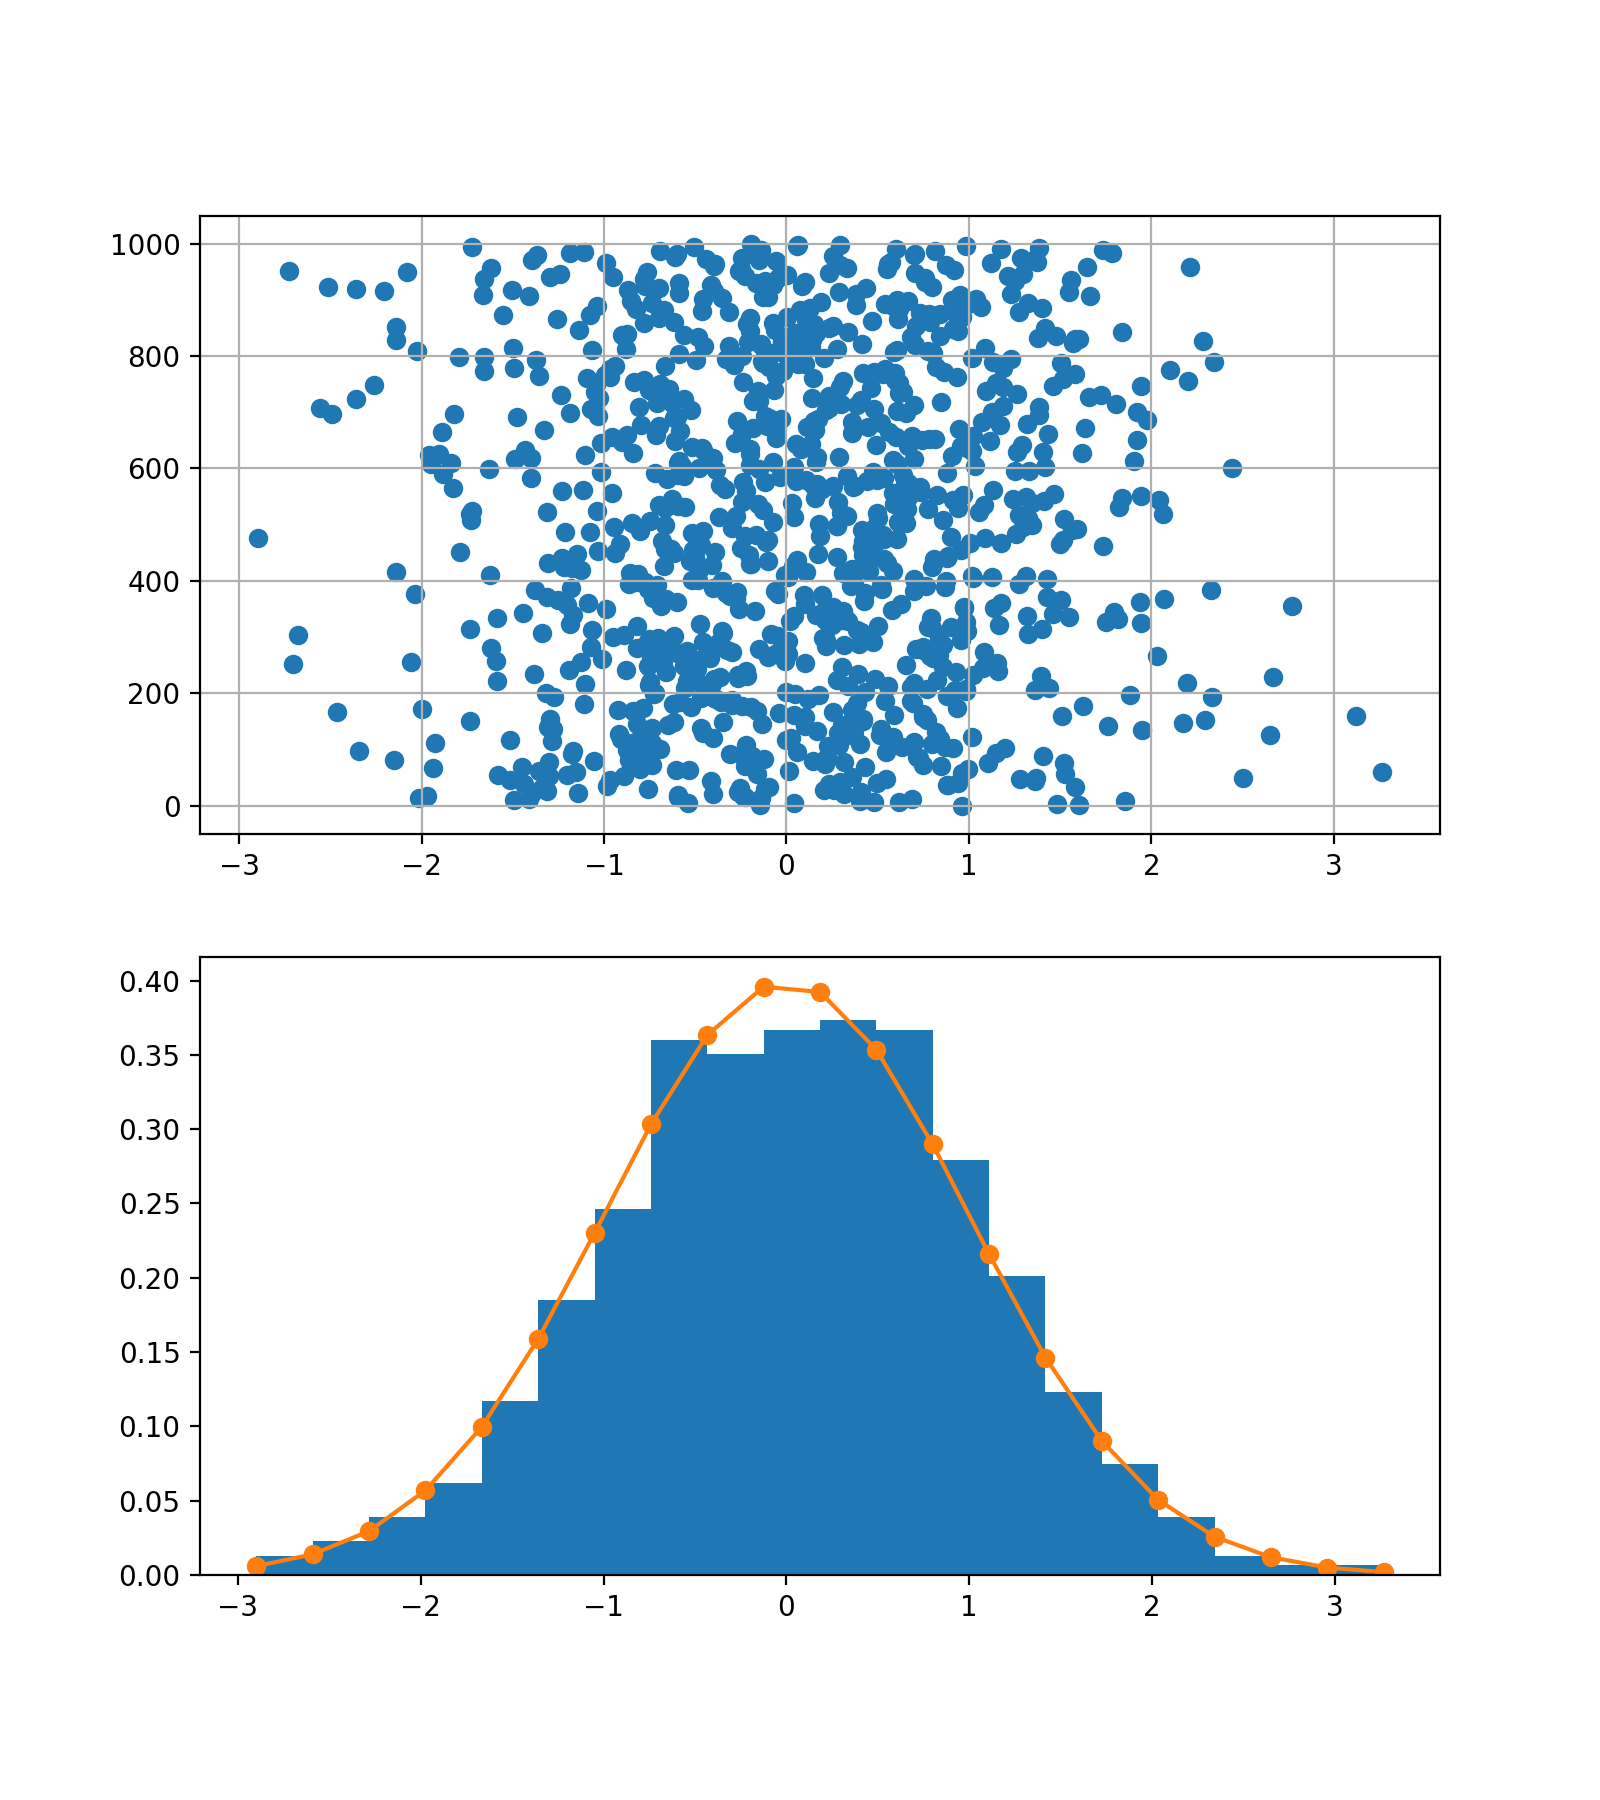
\includegraphics[width=.9\textwidth]{img/rnorm.png}
    \end{column}
  \end{columns}
\end{frame}


\subsection{模型/建模}
\begin{frame}
  \frametitle{统计模型示例}
  \begin{columns}
    \begin{column}{.4\textwidth}
      \begin{block}{单因素方差分析模型}

        $$y_{ij} = \mu + \alpha_i+e_{ij}$$

        \pause
        其中:
      \end{block}
    \end{column}
    \begin{column}{.6\textwidth}
      \begin{description}
      \item [$y_{ij}$] 处理第 $i$ 水平,第 $j$ 重复的观测值
      \item [$\mu$] 整体平均
      \item [$\alpha_i$] 第 $i$ 水平效应
      \item [$e_{ij}$] 每个观测值的随机残差,一般假定 $e_{ij}\stackrel{\mathrm{iid}}{\sim}N(0,\,\sigma_e^2)$
      \end{description}
    \end{column}
  \end{columns}
\end{frame}


\begin{frame}
  \frametitle{统计模型示例}
  \begin{columns}
    \begin{column}{.4\textwidth}
      \begin{block}{``基因组选择''模型}
        $$
        y_i = \mu+{\color{red}\sum_{j=1}^{N_{\mathrm{marker}}}x_{ij}b_j}+e_i
        $$

        \pause

        其中:
      \end{block}
    \end{column}
    \begin{column}{.6\textwidth}
      \begin{description}
      \item [$y_i$] 个体 $i$ 的表型观测值
      \item [$\mu$] 群体平均
      \item [$x_{ij}$] 个体 $i$ 第 $j$ 座位的基因型
      \item [$b_i$] 第 $j$ 座位的基因型值
      \item [$e_i$] 个体 $i$ 的随机残差效应,一般假定独立、同质服从正态分布。
        \pause
      \item [$\displaystyle{\color{red}\sum_{j=1}^{N_{\mathrm{marker}}}x_{ij}b_j}$] {\color{cyan}育种值}
      \end{description}
    \end{column}
  \end{columns}
\end{frame}


% \begin{frame}
%   \frametitle{统计模型示例}
%   \begin{columns}
%     \begin{column}{.4\textwidth}
%       \begin{block}{广义线性模型}
%         $$\mathbf{y=Xb+Zu+e}$$
%         其中:
%       \end{block}
%     \end{column}
%     \begin{column}{.6\textwidth}
%       \begin{description}
%       \item[$\mathbf{y}$] 性状观测值向量
%       \item[$\mathbf{b}$] 固定效应向量
%       \item[$\mathbf{u}$] 随机效应向量
%       \item[$\mathbf{e}$] 随机残差向量,一般独立、同质地服从正态分布
%       \item[$\mathbf{X,\,Z}$] 指示矩阵。指示各 $\mathbf{b}$ 和
%             $\mathbf{u}$ 效应在相应因变量 $y_{ijkl\cdots}$ 中的有无或比例。
%       \end{description}
%     \end{column}
%   \end{columns}
% \end{frame}


\section{线性模型普通最小二乘估计和育种值估计}
\subsection{方程组}
\begin{frame}
  \frametitle{方程组}
  \begin{columns}
    \begin{column}{.4\textwidth}
      今有雉兔同笼,上有三十五头,下有九十四足。问雉兔各几何。

      \flushright{——《孙子算经》}
    \end{column}
    \begin{column}{.6\textwidth}
      \begin{itemize}
      \item 设有 $x_1$ 雉,$x_2$ 兔,则有二元一次方程组:
        %[] to hide the bullets
      \item[] $\displaystyle\begin{array}{rcrcc}
        x_1  & + &  x_2 & = & 35\\
        2x_1 & + & 4x_2 & = & 94\end{array}$
        
        \pause
      \item[] $\displaystyle\left[\begin{array}{cc}
          1&1\\
          2&4
        \end{array}\right]
        \left[\begin{array}{c}
            x_1\\
            x_2
          \end{array}\right]=
        \left[\begin{array}{c}
            35\\
            94
          \end{array}\right]$
        % 注意具体的方程解法是另外一个问题
      \end{itemize}
    \end{column}
  \end{columns}
  \begin{itemize}
    
    \pause
    \vspace{2ex}
    
  \item 若干概念:
    \begin{itemize}
    \item 矩阵、向量、维数/度、方阵、转置、对称阵、秩、满秩、逆矩阵

      \vspace{1ex}
      
    \item 以上:$\mathbf{A\cdot x}=\mathbf{b} \Rightarrow \mathbf{x}=\mathbf{A}^{-1}\cdot\mathbf{b}=\left[\begin{array}{rr}2 & -0.5\\ -1 & 0.5\end{array}\right]\left[\begin{array}{c}35\\ 94 \end{array}\right]=\left[\begin{array}{c}23\\ 12 \end{array}\right]$
      
    \end{itemize}
  \end{itemize}
\end{frame}


\subsection{普通最小二乘 OLS}

\begin{frame}
  \frametitle{普通最小二乘 OLS}
  \begin{columns}
    \begin{column}{.5\textwidth}
      \begin{itemize}
      \item 简单如单因子方差分析:
        \begin{itemize}
        \item $y_{ij}=\mu+\alpha_i+e_{ij}$
          \begin{itemize}
          \item 一个观测值一个方程
          \item $e_{ij}$ 在每个方程中都有,且各不相同
          \item 整个方程组还包括总的水平数和 1 个群体平均
          \item 未知数个数超过方程个数
          \end{itemize}
        \item $\Rightarrow$ 方程无解
        \end{itemize}
      \end{itemize}
    \end{column}
    \pause
    \begin{column}{.5\textwidth}
      \begin{itemize}
      \item 最小二乘估计
        \begin{itemize}
        \item 找到这样一组参数 $\theta$ 的估计值 $\hat\theta$,使得:
          \begin{itemize}
          \item 残差 $e$,即估计值 $\hat{y}$ 与观测值 $y$ 之差,的平方和最小。
          \item 用式子表示:
            $$\hat\theta=\arg\min_{\theta}\sum_{i=1}^n(f_{\theta}(x_i)-y_i)^2$$
          \end{itemize}
        \item 亦即,观测值与估计值之间的欧几里得距离最小。
        \end{itemize}
      \end{itemize}
    \end{column}
  \end{columns}
\end{frame}


\begin{frame}
  \frametitle{普通最小二乘 OLS}
  \begin{columns}
    \begin{column}{.5\textwidth}
      $$\hat\theta=\arg\min_{\theta}\sum_{i=1}^n\left(f_{\theta}(x_i)-y_i\right)^2$$

    \end{column}
    
    \begin{column}{.5\textwidth}
      \begin{itemize}
      \item $\displaystyle\hat{\theta}=\arg\min_{\theta}L$: Arguments of the minimum of function $L$
      \item 二次型有解析最小值
      \item 容易推导和计算
      \item 鲁棒、稳健
      \item 属于一种优化估计
      \end{itemize}
    \end{column}
  \end{columns}
\end{frame}


\subsection{推导}
\begin{frame}
  \frametitle{优化估计}
  \begin{columns}
    \begin{column}{.5\textwidth}
      \begin{block}{什么是优化估计}
        \hspace{2em}选择模型的参数 $\hat\theta$,使得模型对观测值有最优解释。
        $$\hat\theta=\arg\min_{\theta}L_i(f_{\theta}(x_i,\theta), y_i)$$
      \end{block}
    \end{column}
    \pause
    \begin{column}{.5\textwidth}
      \begin{block}{三个概念}
        \hspace{2em}模型、目标、优化
      \end{block}
      \begin{block}{最小二乘的优化估计}
        $$\hat\theta=\arg\min_{\theta}\sum_{i-1}^n(f_{\theta}(x_i)-y_i)^2$$
      \end{block}
    \end{column}
  \end{columns}
\end{frame}


\begin{frame}
  \begin{columns}
    \begin{column}{.4\textwidth}
      \begin{itemize}
      \item 模型
      \end{itemize}
      $$y_i = \sum_{j=1}^{m}x_{ij}\theta_j+e_i$$
    \end{column}
    \pause
    \begin{column}{.6\textwidth}
      \begin{itemize}
      \item 方程组表示
      \end{itemize}
      $$
      \left[\begin{array}{c}
          y_1\\
          \vdots\\
          y_n
        \end{array}\right]
      =
      \left[\begin{array}{ccc}
          x_{11} & \cdots & x_{1m}\\
          \vdots & \ddots & \vdots\\
          x_{n1} & \cdots & x_{nm}
        \end{array}\right]
      \left[\begin{array}{c}
          \theta_1\\
          \vdots\\
          \theta_m
        \end{array}\right]
      +
      \left[\begin{array}{c}
          e_1\\
          \vdots\\
          e_n
        \end{array}\right]
      $$
      
      \begin{itemize}
      \item 或者
      \end{itemize}
      $$\mathbf{y=X\theta+e}$$
    \end{column}
  \end{columns}
\end{frame}


\begin{frame}
  \frametitle{优化估计的目标和优化}
  \begin{columns}
    \begin{column}{.5\textwidth}
      \begin{block}{目标}
        \hspace{2em}令 $\sum(e_i^2)$ 最小。

        \hspace{2em}或者说,我们要寻找这样的参数估计值 $\hat{\theta}$, 它们使得 $\sum(y_i-\mathbf{x\theta})^2$, 或者 $\mathbf{(y-X\theta)'(y-X\theta)}$,最小。
      \end{block}
    \end{column}
    \pause
    \begin{column}{.5\textwidth}
      \begin{block}{优化}
        \hspace{2em}将左边二次式对 $\mathbf{\theta}$ 的一阶导数为零时有唯一解。
      \end{block}
    \end{column}
  \end{columns}
\end{frame}


\begin{frame}
  \frametitle{示例 — 当 $\theta$ 中仅含一个参数 $b$}
  \begin{columns}
    \begin{column}{0.5\textwidth}
      \begin{block}{优化函数 $L$}
        
        $$
        \begin{array}{rcl}
          L & = & \sum_i^n(y_i-x_ib)^2\\
          & = & \sum_i^n(y_i^2-2x_iy_ib+x_i^2b^2)
        \end{array}
        $$
        
      \end{block}
    \end{column}
    \pause
    \begin{column}{.5\textwidth}
      \begin{block}{对 $b$ 求导}
        $$L'=\sum_i^n(2x_i^2b-2x_iy_i)$$
      \end{block}
      \begin{block}{令优化函数一阶导数 $L'=0$}
        $$b=\frac{\sum x_iy_i}{\sum x_i^2}$$
      \end{block}
    \end{column}
  \end{columns}
\end{frame}


\begin{frame}
  \frametitle{示例 — 当 $\theta$ 中仅含两个参数$b_1,\,b_2$}
  \begin{block}{优化函数 $L$}
    $$
    \begin{array}{ccl}
      L & = & \sum_i^n(y_i-x_{i1}b_1-x_{i2}b_2)^2\\
      & = & \sum_i^n(y_i^2 + x_{i1}^2b_1^2 + x_{i2}^2b_2^2\\
      &   & \quad + 2x_{i1}x_{i2}b_1b_2 - 2x_{i1}y_ib_1 - 2x_{i2}y_ib_2)^2
    \end{array}
    $$
    
  \end{block}
  \pause
  \begin{block}{分别对 $b_1$ 和 $b_2$ 求导}
    $$
    \left\{\begin{array}{rcl}
    L_{b_1}' & = & \sum(2x_{i1}^2b_1+2x_{i1}x_{i2}b_2-2x_{i1}y_i)\\
    L_{b_2}' & = & \sum(2x_{i2}^2b_2+2x_{i1}x_{i2}b_1-2x_{i2}y_i)
    \end{array}\right.
    $$
  \end{block}
\end{frame}


\begin{frame}
  \frametitle{示例 — 当 $\theta$ 中仅含两个参数$b_1,\,b_2$}
  \begin{block}{令 $L_{b_1}' = L_{b_2}' = 0$}
    $$
    \left\{\begin{array}{rcrcl}
    (\sum x_{i1}^2)b_1 &+& (\sum x_{i1}x_{i2}) b_2 &=& \sum x_{i1}y_i\\
    (\sum x_{i1}x_{i2})b_1 &+& (\sum x_{i2}^2)b_2 &=& \sum x_{i2}y_i
    \end{array}\right.
    $$
  \end{block}
  \pause
  \begin{block}{显而易见,以上即方程组}
    
    $$
    \left[\begin{array}{ll}
        \sum x_{i1}^2 & \sum x_{i1}x_{i2}\\
        \sum x_{i1}x_{i2} & \sum x_{i2}^2
      \end{array}\right]
    \left[\begin{array}{c}
        b_1\\
        b_2
      \end{array}\right] = (\mathbf{X'X})\mathbf{b} = \mathbf{X'y}
    $$
    
  \end{block}
\end{frame}


\begin{frame}
  \frametitle{线性模型普通最小二乘估计}
  \begin{block}{该方程组解}
    $$\hat{\theta} = \hat{\mathbf{b}} = (\mathbf{X}'\mathbf{X})^{-1}\mathbf{X'y}$$
  \end{block}
\end{frame}


\subsection{模拟示例}
\begin{frame}
  \frametitle{模拟}
  \begin{itemize}
  \item 一个最小二乘估计育种值的模拟
  \item 见 {\color{cyan}day-1-least-square.ipynb}
  \end{itemize}
\end{frame}
\end{document}


%“种、料、繁、舍、病、管”。第一个种,即品种;第二个料,即饲料营养;第三个繁,即繁殖技术;第四个舍,即猪舍环境和设备;第五个病,即疫病防控;第六个管理。
% 中国农业大学张忠诚教授
